%%%%%%%%%%%%%%%%%%%%%%%%%%%%%%%%%%%%
%                                  %
% Titre  : s_i.tex                 %
% Sujet  : Manuel de l'utilisateur %
%          du projet 'Scotch'      %
%          Introductions           %
% Auteur : Francois Pellegrini     %
%                                  %
%%%%%%%%%%%%%%%%%%%%%%%%%%%%%%%%%%%%

\section{Introduction}

\subsection{Static mapping}

The efficient execution of a parallel program on a parallel machine
requires that the communicating processes of the program be assigned
to the processors of the machine so as to minimize its overall running
time.
When processes have a limited duration and their logical dependencies
are accounted for, this optimization problem is referred to as
\emph{scheduling}.
When processes are assumed to coexist simultaneously for the entire
duration of the program, it is referred to as \emph{mapping}. It
amounts to balancing the computational weight of the processes among the
processors of the machine, while reducing the cost of communication by
keeping intensively inter-communicating processes on nearby
processors.
In most cases, the underlying computational structure of the parallel
programs to map can be conveniently modeled as a graph in which
vertices correspond to processes that handle distributed pieces of
data, and edges reflect data dependencies. The mapping problem can
then be addressed by assigning processor labels to the vertices of the
graph, so that all processes assigned to some processor are loaded and
run on it.
In a SPMD context, this is equivalent to the \emph{distribution\/}
across processors of the data structures of parallel programs; in this
case, all pieces of data assigned to some processor are handled by a
single process located on this processor.

A mapping is called \emph{static\/} if it is computed prior to the
execution of the program. Static mapping is NP-complete in the general
case~\cite{gajo79}. Therefore, many studies have been carried out in
order to find sub-optimal solutions in reasonable time, including
the development of specific algorithms for common topologies such
as the hypercube~\cite{errasa90,hamm92}.
When the target machine is assumed to have a communication network in
the shape of a complete graph, the static mapping problem turns into
the \emph{partitioning\/} problem, which has also been intensely
studied~\cite{basi94,hele93a,kaku95a,kaku95c,posili90}.
However, when mapping onto parallel machines the communication network
of which is not a bus, not accounting for the topology of the target
machine usually leads to worse running times, because simple cut
minimization can induce more expensive long-distance
communication~\cite{hamm92,wacrevjo95}.

\subsection{Sparse matrix ordering}

Many scientific and engineering problems can be modeled by sparse linear
systems, which are solved either by iterative or direct methods.
To achieve efficiency with direct methods, one must minimize the
fill-in induced by factorization. This fill-in is a direct consequence of
the order in which the unknowns of the linear system are numbered,
and its effects are critical both in terms of memory and computation costs.
\\

An efficient way to compute fill reducing orderings of symmetric
sparse matrices is to use recursive nested dissection~\cite{geli81}.
It amounts to computing a vertex set~$S$ that separates the graph into
two parts~$A$ and~$B$, ordering $S$ with the highest indices that are
still available, and proceeding recursively on parts~$A$ and~$B$ until
their sizes become smaller than some threshold value. This ordering
guarantees that, at each step, no non-zero term can appear in the
factorization process between unknowns of~$A$ and unknowns of~$B$.

The main issue of the nested dissection ordering algorithm is thus to
find small vertex separators that balance the remaining subgraphs as
evenly as possible, in order to minimize fill-in and to increase
concurrency in the factorization process.

\subsection{Contents of this document}

This document describes the capabilities and operations of \scotch,
a software package devoted to static mapping, graph and mesh
partitioning, and sparse matrix block ordering.
\scotch\ allows the user to map efficiently any kind of weighted process
graph onto any kind of weighted architecture graph, and provides high-quality
block orderings of sparse matrices.
The rest of this manual is organized as follows.
Section~\ref{sec-project} presents the goals of the \scotch\ project.
Sections~\ref{sec-algo-map} and~\ref{sec-algo-order} outline the most
important aspects of the mapping and ordering algorithms that it
implements, respectively.
Section~\ref{sec-changes} summarizes the most important changes between
version~\textsc{5.0} and previous versions.
Section~\ref{sec-file} defines the formats of the files used in \scotch,
section~\ref{sec-prog} describes the programs of the
\scotch\ distribution, and section~\ref{sec-lib} defines the interface
and operations of the \libscotch\ library.
Section~\ref{sec-install} explains how to obtain and install the
\scotch\ distribution.
Finally, some practical examples are given in
section~\ref{sec-examples}, and instructions on how to implement new
methods in the \libscotch\ library are provided in
section~\ref{sec-coding}.

\section{The \scotch\ project}
\label{sec-project}

\subsection{Description}

\scotch\ is a project carried out at the \textit{Laboratoire Bordelais de
Recherche en Informatique\/} (LaBRI) of the Universit\'e de Bordeaux and
within the Tadaam team-project of INRIA Bordeaux Sud-Ouest. Its goal
is to study the application of graph theory to scientific computing.

It focused first on static mapping, and has resulted in the
development of the Dual Recursive Bipartitioning (or DRB) mapping
algorithm and in the study of several graph bipartitioning
heuristics~\cite{pell94a}, all of which have been implemented in the
\scotch\ software package~\cite{pero96a}. Then, it focused on the
computation of high-quality vertex separators for the ordering of
sparse matrices by nested dissection, by extending the work that has
been done on graph partitioning in the context of static
mapping~\cite{pero97a,peroam99}. The ordering
capabilities of \scotch\ have then been extended to native mesh structures,
thanks to hypergraph partitioning algorithms. Diffusion-based graph
partitioning methods have also been added~\cite{chpe06a,pell07b}.

Version \textsc{5.0} of \scotch\ was the first one to comprise parallel
graph ordering routines. The parallel features of \scotch\ are referred
to as \ptscotch\ (``\emph{Parallel Threaded \scotch}''). While both
packages share a significant amount of code, because
\ptscotch\ transfers control to the sequential routines of the
\libscotch\ library when the subgraphs on which it operates are
located on a single processor, the two sets of routines have a
distinct user's manual. Readers interested in the parallel features
of \scotch\ should refer to the \emph{\ptscotch\ \textsc{\scotchver}
User's Guide}~\scotchcitepuser.

Version \textsc{6.0} of \scotch\ is oriented towards the development of
new features, namely graph repartitioning and
remapping~\cite{fope11a}. A whole set of direct $k$-way graph
partitioning and mapping algorithms has also been implemented.
Also, new target architectures have been created, to allow \scotch\ to
map efficiently onto parts of regular target
architectures~\cite{pellegrini:hal-01671156}, as it is the case when
considering a potentially non-connected partition of a big machine, as
provided by a batch scheduler.

\subsection{Availability}

Starting from version \textsc{4.0}, which has been developed at INRIA
within the ScAlApplix project, \scotch\ is available under a dual
licensing basis. On the one hand, it is downloadable from the
\scotch\ web page as free/libre software, to all interested parties
willing to use it as a library or to contribute to it as a testbed for
new partitioning and ordering methods. On the other hand, it can also
be distributed, under other types of licenses and conditions, to
parties willing to embed it tightly into closed, proprietary software.
\\

The free/libre software license under which \scotch\ \textsc{\scotchver}
is distributed is the CeCILL-C license~\cite{cecill}, which has
basically the same features as the GNU LGPL (``\textit{Lesser General
Public License}''): ability to link the code as a library to any
free/libre or even proprietary software, ability to modify the code
and to redistribute these modifications. Version \textsc{4.0} of
\scotch\ was distributed under the LGPL itself.
\\

Please refer to section~\ref{sec-install} to see how to obtain the
free/libre distribution of \scotch.

\section{Static mapping algorithms}
\label{sec-algo-map}

The parallel program to be mapped onto the target architecture is modeled
by a valuated unoriented graph $S$ called \emph{source graph\/} or
\emph{process graph}, the vertices of which represent the processes of the
parallel program, and the edges of which the communication channels between
communicating processes.
Vertex- and edge- valuations associate with every vertex $v_S$ and every
edge $e_S$ of $S$ integer numbers $w_S(v_S)$ and $w_S(e_S)$ which
estimate the computation weight of the corresponding process
and the amount of communication to be transmitted on the channel,
respectively.

The target machine onto which is mapped the parallel program is also
modeled by a valuated unoriented graph $T$ called \emph{target graph\/}
or \emph{architecture graph}.
Vertices $v_T$ and edges $e_T$ of $T$ are assigned integer weights
$w_T(v_T)$ and $w_T(e_T)$, which estimate the computational power of the
corresponding processor and the cost of traversal of the inter-processor
link, respectively.

A \emph{mapping} from $S$ to $T$ consists of two applications
$\too{S,T} : V(S) \rghta V(T)$ and
$\roo{S,T} : E(S) \rghta {\cal P}(E(T))$,
where ${\cal P}(E(T))$ denotes the set of all simple loopless paths which
can be built from $E(T)$.
$\too{S,T}(v_S) = v_T$ if process $v_S$ of $S$ is mapped onto processor
$v_T$ of $T$, and $\roo{S,T}(e_S) = \{ e^1_T, e^2_T, \ldots, e^n_T \}$ if
communication channel $e_S$ of $S$ is routed through communication links
$e^1_T$, $e^2_T$, \ldots, $e^n_T$ of $T$.
$|\roo{S,T}(e_S)|$ denotes the dilation of edge $e_S$, that is, the number of
edges of $E(T)$ used to route $e_S$.

\subsection{Cost function and performance criteria}

The computation of efficient static mappings requires an \emph{a priori\/}
knowledge of the dynamic behavior of the target machine with respect to
the programs which are run on it.
This knowledge is synthesized in a \emph{cost function}, the nature of which
determines the characteristics of the desired optimal mappings.
The goal of our mapping algorithm is to minimize some communication cost
function, while keeping the load balance within a specified tolerance.
The communication cost function $f_C$ that we have chosen is the sum,
for all edges, of their dilation multiplied by their weight:
\bn
f_C(\too{S,T},\roo{S,T})
\eqdef \hspace*{-0.25cm}\sum\limits_{e_S\in E(S)}\hspace*{-0.25cm}
w_S(e_S)\,|\roo{S,T}(e_S)|\enspace.
\en
This function, which has already been considered by several authors for
hypercube target topologies~\cite{errasa90,hamm92,hele94b}, has several
interesting properties:
it is easy to compute, allows incremental updates performed by
iterative algorithms, and
its minimization favors the mapping of intensively intercommunicating
processes onto nearby processors;
regardless of the type of routing implemented on the target machine
(store-and-forward or cut-through), it models the traffic on the
interconnection network and thus the risk of congestion.

The strong positive correlation between values of this function and
effective execution times has been experimentally verified by
Hammond~\cite{hamm92} on the CM-2, and by Hendrickson and
Leland~\cite{hele94a} on the nCUBE~2.
\hfill~\\

The quality of mappings is evaluated with respect to the criteria for
quality that we have chosen: the balance of the computation load across
processors, and the minimization of the inter-processor communication cost
modeled by function~$f_C$. These criteria lead to the definition of
several parameters, which are described below.

For load balance, one can define $\mmap$, the average load per
computational power unit (which does not depend on the mapping), and
$\dmap$, the load imbalance ratio, as\\[-0.5em]
\bn
\mmap \eqdef
{\sum\limits_{v_S \in V(S)} w_S(v_S) \over
 \sum\limits_{v_T \in V(T)} w_T(v_T)}
\hspace*{2.5em}\mbox{~and~}
\en
\bn
\dmap \eqdef
{\sum\limits_{v_T \in V(T)}
   \left|\left(\!\!{1 \over w_T(v_T)}\hspace*{-0.3em}
         \sum\limits_{\scriptsize
                      \shortstack{$v_S \in V(S)$\\[-0.2em]
                                  $\too{S,T}(v_S) = v_T$}}
         \hspace*{-0.2em} w_S(v_S)\!\!\right)\:-\:\mmap\right| \over
\sum\limits_{v_S \in V(S)} w_S(v_S)}\enspace.
\en
However, since the maximum load imbalance ratio is provided by the user in
input of the mapping, the information given by these parameters is of little
interest, since what matters is the minimization of the communication cost
function under this load balance constraint.

For communication, the straightforward parameter to consider is $f_C$.
It can be normalized as $\mexp$, the average edge expansion, which can
be compared to $\mdil$, the average edge dilation; these are defined
as\\[-1.3em]
\bn
\mexp \eqdef {f_C \over \sum\limits_{e_S \in E(S)} w_S(e_S)}
\hspace*{2.5em}\mbox{~and~}\hspace*{2.5em}
\mdil \eqdef {\sum\limits_{e_S \in E(S)}|\roo{S,T}(e_S)| \over |E(S)|}
\enspace.
\en
$\dexp \eqdef {\mexp \over \mdil}$ is smaller than $1$ when the mapper
succeeds in putting heavily intercommunicating processes closer to each other
than it does for lightly communicating processes; they are equal if all edges
have same weight.

\subsection{The Dual Recursive Bipartitioning algorithm}
\label{sec-algo-drb}

This mapping algorithm, which is the primary way to compute initial
static mappings, uses a \emph{divide and conquer\/} approach to
recursively allocate subsets of processes to subsets of
processors~\cite{pell94a,pero96b}. It starts by considering a set of
processors, also called \emph{domain}, containing all the processors of
the target machine, and with which is associated the set of all the
processes to map.  At each step, the algorithm bipartitions a yet
unprocessed domain into two disjoint subdomains, and calls a
\emph{graph bipartitioning algorithm\/} to split the subset of
processes associated with the domain across the two subdomains, as
sketched in the following.

\noi
{\renewcommand{\baselinestretch}{0.95}\footnotesize\tt {%
\begin{verbatim}
mapping (D, P)
Set_Of_Processors  D;
Set_Of_Processes   P;
{
  Set_Of_Processors  D0, D1;
  Set_Of_Processes   P0, P1;

  if (|P| == 0) return;  /* If nothing to do.     */
  if (|D| == 1) {        /* If one processor in D */
    result (D, P);       /* P is mapped onto it.  */
    return;
  }

  (D0, D1) = processor_bipartition (D);
  (P0, P1) = process_bipartition   (P, D0, D1);
  mapping (D0, P0);      /* Perform recursion. */
  mapping (D1, P1);
}
\end{verbatim}}}

\noi
The association of a subdomain with every process defines a \emph{partial
mapping\/} of the process graph. As bipartitionings are performed,
the subdomain sizes decrease, up to give a complete mapping when all
subdomains are of size~one.
\\

The above algorithm lies on the ability to define five main objects:
\begin{itemize}
\item
a \emph{domain structure}, which represents a set of processors in the target
architecture;
\item
a \emph{domain bipartitioning function}, which, given a domain, bipartitions
it in two disjoint subdomains;
\item
a \emph{domain distance function}, which gives, in the target graph, a measure
of the distance between two disjoint domains. Since domains may not be convex
nor connected, this distance may be estimated.
However, it must respect certain homogeneity properties, such as
giving more accurate results as domain sizes
decrease~\cite{pero96b,pellegrini:hal-01671156}.
The domain distance function is used by the graph bipartitioning algorithms
to compute the communication function to minimize, since it allows the mapper
to estimate the dilation of the edges that link vertices which belong to
different domains.
Using such a distance function amounts to considering that all routings
will use shortest paths on the target architecture, which is how most
parallel machines actually do.
We have thus chosen that our program would not provide routings for the
communication channels, leaving their handling to the communication system of
the target machine;
\item
a \emph{process subgraph structure}, which represents the subgraph induced by a
subset of the vertex set of the original source graph;
\item
a \emph{process subgraph bipartitioning function}, which bipartitions subgraphs
in two disjoint pieces to be mapped onto the two subdomains computed by
the domain bipartitioning function.
\end{itemize}
All these routines are seen as black boxes by the mapping program, which can
thus accept any kind of target architecture and process bipartitioning
functions.

\subsubsection{Partial cost function}

The production of efficient complete mappings requires that all graph
bipartitionings favor the criteria that we have chosen.
Therefore, the bipartitioning of a subgraph~$S'$ of $S$ should maintain
load balance within the user-specified tolerance, and minimize the
\emph{partial\/} communication cost function $f'_C$, defined as
\bn
f'_C(\too{S,T},\roo{S,T}) \eqdef
\hspace*{-0.45cm}\sum\limits_{\mbox{\scriptsize
             \shortstack{$v\in V(S')$\\
                         $\{v,v'\}\in E(S)$}}}\hspace*{-0.45cm}
w_S(\{v,v'\})\,|\roo{S,T}(\{v,v'\})|\enspace,
\en
which accounts for the dilation of edges internal to subgraph~$S'$ as well as
for the one of edges which belong to the cocycle of $S'$, as shown in
Figure~\ref{fig-bipcost}.
Taking into account the partial mapping results issued by previous
bipartitionings makes it possible to avoid local choices that
might prove globally bad, as explained below.
This amounts to incorporating additional constraints to the standard graph
bipartitioning problem, turning it into a more general optimization problem
termed \emph{skewed graph partitioning\/} by some authors~\cite{heledr97}.

\begin{figure}[hbt]
\hfill
\parbox[b]{4.9cm}{
\hfill
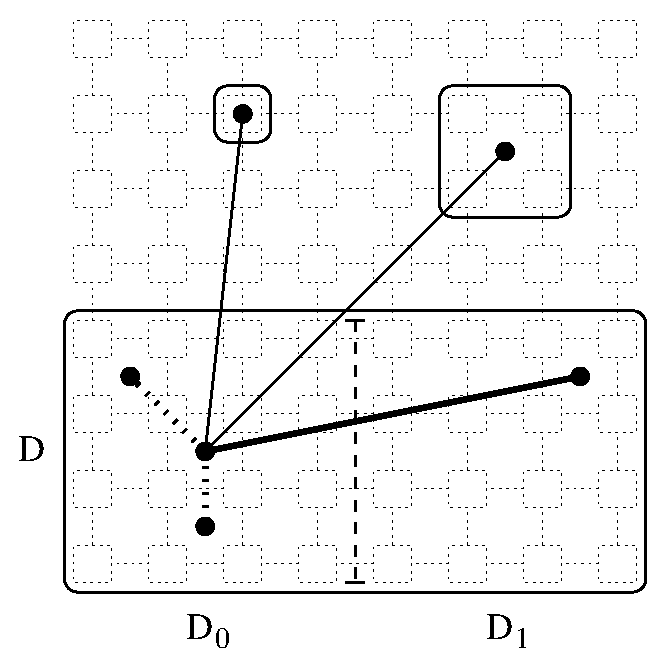
\includegraphics[scale=0.40]{s_f_rua.eps}
\hfill\\
\textbf{a.} Initial position.
}\ \hfill\
\parbox[b]{4.9cm}{
\hfill
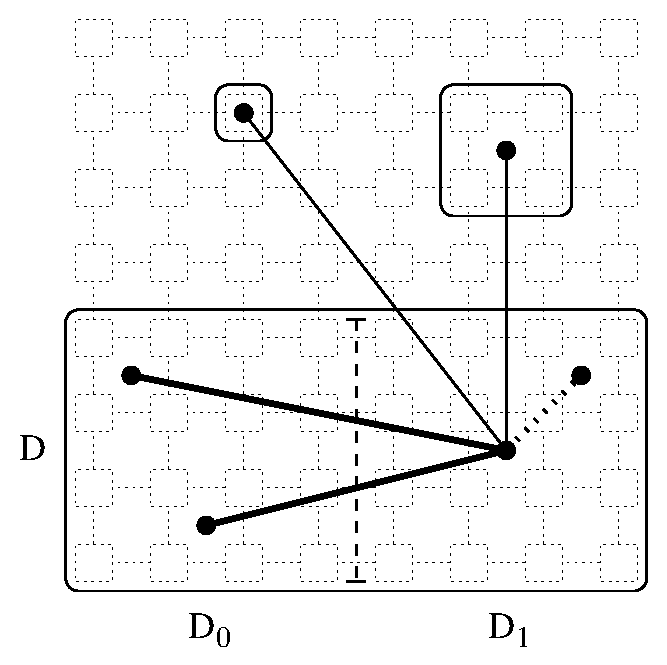
\includegraphics[scale=0.40]{s_f_rub.eps}
\hfill\\
\textbf{b.} After one vertex is moved.
}\hfill\
\caption%
{Edges accounted for in the partial communication cost function when
 bipartitioning the subgraph associated with domain~$D$ between
 the two subdomains $D_0$ and $D_1$ of~$D$.
 Dotted edges are of dilation zero, their two ends being mapped onto the
 same subdomain. Thin edges are cocycle edges.}
\label{fig-bipcost}
\end{figure}

\subsubsection{Execution scheme}

From an algorithmic point of view, our mapper behaves as a greedy algorithm,
since the mapping of a process to a subdomain is never reconsidered, and
at each step of which iterative algorithms can be applied.
The double recursive call performed at each step induces a recursion scheme
in the shape of a binary tree, each vertex of which corresponds to a
bipartitioning job, that is, the bipartitioning of both a domain and
its associated subgraph.

In the case of depth-first sequencing, as written in the above sketch,
bipartitioning jobs run in the left branches of the tree have no information
on the distance between the vertices they handle and neighbor vertices to be
processed in the right branches.
On the contrary, sequencing the jobs according to a by-level (breadth-first)
travel of the tree allows any bipartitioning job of a given level to
have information on the subdomains to which all the processes have been
assigned at the previous level.
Thus, when deciding in which subdomain to put a given process, a
bipartitioning job can account for the communication costs induced by
its neighbor processes, whether they are handled by the job itself or not,
since it can estimate in $f'_C$ the dilation of the corresponding edges.
This results in an interesting feedback effect: once an edge has been kept
in a cut between two subdomains, the distance between its end vertices will
be accounted for in the partial communication cost function to be minimized,
and following jobs will be more likely to keep these vertices close to
each other, as illustrated in Figure~\ref{fig-biprub}.
\begin{figure}[hbt]
\hfill
\parbox[b]{5.2cm}{
\hfill
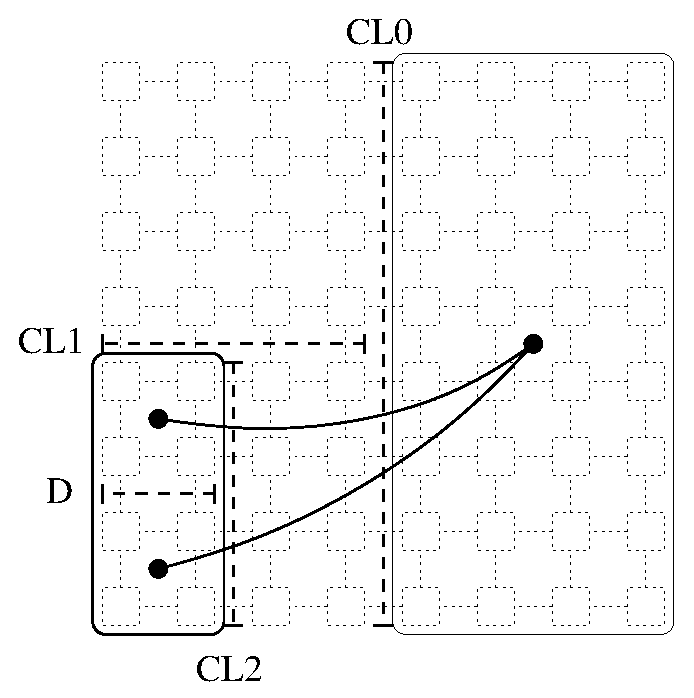
\includegraphics[scale=0.40]{s_f_run.eps}
\hfill\\
\textbf{a.} Depth-first sequencing.
}\ \hfill\
\parbox[b]{5.2cm}{
\hfill
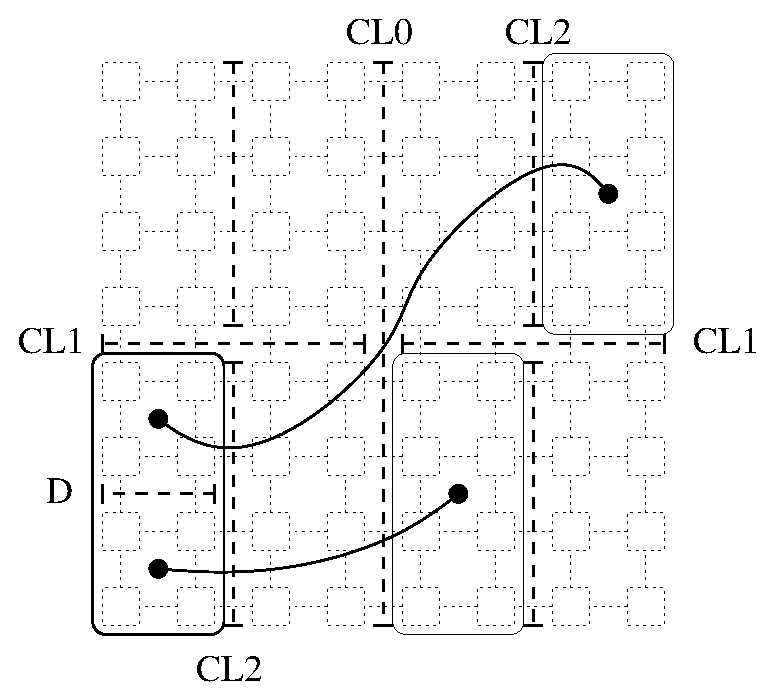
\includegraphics[scale=0.40]{s_f_ruy.eps}
\hfill\\
\textbf{b.} Breadth-first sequencing.
}\hfill\ %
\caption%
{Influence of depth-first and breadth-first sequencings on the
 bipartitioning of a domain~$D$ belonging to the leftmost branch of
 the bipartitioning tree.
 With breadth-first sequencing, the partial mapping data regarding vertices
 belonging to the right branches of the bipartitioning tree are more
 accurate (C.L. stands for ``Cut Level'').}
\label{fig-biprub}
\end{figure}
The relative efficiency of depth-first and breadth-first sequencing schemes
with respect to the structure of the source and target graphs is discussed
in~\cite{pero96b}.

\subsubsection{Clustering by mapping onto variable-sized architectures}
\label{sec-algo-variable}
\index{Architecture|Variable-sized!see Clustering}
\index{Clustering}

Several constrained graph partitioning problems can be modeled as
mapping the problem graph onto a target architecture, the number of
vertices and topology of which depend dynamically on the structure of
the subgraphs to bipartition at each step.

Variable-sized architectures are supported by the DRB algorithm in the
following way: at the end of each bipartitioning step, if any of the
variable subdomains is empty (that is, all vertices of the subgraph
are mapped only to one of the subdomains), then the DRB process stops
for both subdomains, and all of the vertices are assigned to their
parent subdomain; else, if a variable subdomain has only one vertex
mapped onto it, the DRB process stops for this subdomain, and the
vertex is assigned to it.

The moment when to stop the DRB process for a specific subgraph can be
controlled by defining a bipartitioning strategy that checks the
validity of a criterion at each bipartitioning step (see for instance
Section~\ref{sec-lib-func-stratgraphclusterbuild}), and maps all of
the subgraph vertices to one of the subdomains when it becomes false.

\subsection{Static mapping methods}
\label{sec-algo-map-methods}

The core of our static mapping software uses graph mapping methods as
black boxes. It maintains an internal image of the current mapping,
which records the target vertex index onto which each of the source
graph vertices is mapped. It is therefore possible to apply several
mapping methods in sequence, such that the first method computes an
initial mapping to be further refined by the following methods, thus
enabling us to define \emph{static mapping strategies}. The currently
implemented static mapping methods are listed below.

\begin{itemize}
\iteme[\textbf{Multilevel}]\label{sec-algo-mle}
This framework, which has been studied by several
authors~\cite{basi94,hele93b,kaku95a} and should be considered as a strategy
rather than as a method since it uses other methods as parameters, repeatedly
reduces the size of the graph to map by finding matchings that
collapse vertices and edges, computes a mapping of the coarsest
graph obtained, and prolongs the result back to the original graph,
as shown in Figure~\ref{fig-multiproc}.
\begin{figure}[hbt]
~\hfill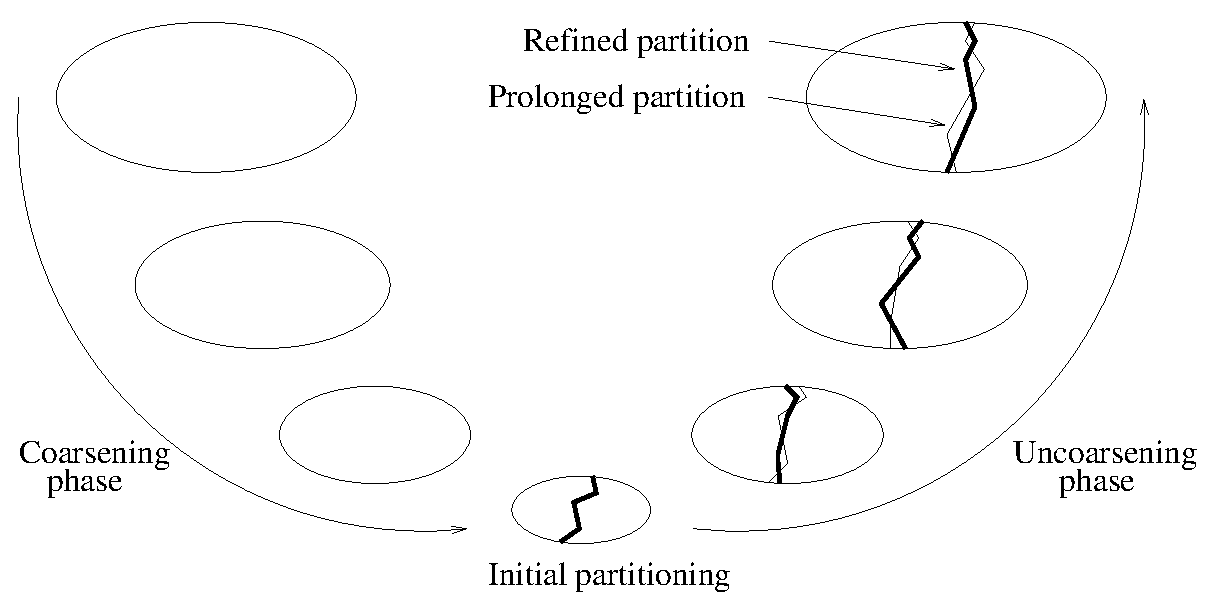
\includegraphics[scale=0.50]{s_f_mult.eps}\hfill\ ~
\caption%
{The multilevel partitioning process. In the uncoarsening phase, the light
 and bold lines represent for each level the prolonged partition obtained
 from the coarser graph, and the partition obtained after refinement,
 respectively.}
\label{fig-multiproc}
\end{figure}
The multilevel method, when used in conjunction with some local
optimization methods to refine the projected partitions at every
level, usually leads to a significant improvement in quality with
respect to methods operating only on the finest graph. By coarsening
the graphs, the multilevel algorithm broadens the scope of local
optimization algorithms: it makes possible for them to account for
topological structures of the original graph that would else be of a
too high level for them to be encompassed in their local optimization
process.
\iteme[\textbf{Band}]\label{sec-algo-band}
Like the multilevel method above, the band method is a framework, in
the sense that it does not itself compute partitions, but rather helps
other partitioning algorithms perform better. It is a refinement
algorithm which, from a given initial partition, extracts a band graph
of given width (which only contains graph vertices that are at most at
this distance from the frontiers of the parts), calls a partitioning
strategy on this band graph, and projects back the refined partition
on the original graph. This method was designed to be able to use
expensive partitioning heuristics, such as genetic algorithms, on
large graphs, as it dramatically reduces the problem space by several
orders of magnitude. However, it was found that, in a multilevel
context, it also improves partition quality, by coercing partitions in
a problem space that derives from the one which was globally defined
at the coarsest level, thus preventing local optimization refinement
algorithms to be trapped in local optima of the finer
graphs~\cite{chpe06a}.
\iteme[\textbf{Fiduccia-Mattheyses}]
This is a direct $k$-way version of the traditional Fiduccia-Mattheyses
heuristics used for computing bipartitions, that will be presented in
the next section. By default, boundary vertices can only be moved to
parts to which at least one of their neighbors belong.
\iteme[\textbf{Diffusion}]
This is also a $k$-way version of an algorithm that has been first used
in the context of bipartitioning, and which will be presented in the
next section. The $k$-way version differs from the latter as it diffuses
$k$ sorts of liquids rather than just two as in the bipartitioning case.
\iteme[\textbf{Exactifier}]\label{sec-algo-map-exact}
This greedy algorithm refines its input mapping so as to reduce load
imbalance as much as possible. Since this method does not consider
load balance minimization, its use should be restricted to cases where 
achieving load balance is critical and where recursive
bipartitioning may fail to achieve it. It is especially the case when
vertex loads are very irregular: some subdomains may receive only a
few heavy vertices, yielding load balance artifacts when no light
vertices are locally available to compensate.

Graph vertices are sorted by decreasing weights, and considered in
turn. If the current vertex can fit in its initial part without
causing imbalance by excess, it is added to it, and the algorithm goes
on. Else, a candidate part is found by exploring other subdomains in
an order based on an implicit recursive bipartitioning of the
architecture graph. Consequently, such vertices will be placed in
subdomains that tend to be as close as possible to the original
location of the vertex. This method is most likely to result in
disconnected parts.
\iteme[\textbf{Dual recursive bipartitioning}]
This algorithm implements the dual recursive bipartitioning algorithm
that has been presented in Section~\ref{sec-algo-drb}. The DRB
algorithms can be used either directly on the original graph to
partition, or on the coarsest graph yielded by the direct $k$-way
multilevel framework. It uses graph bipartitioning methods, described
below, to compute its bipartitions.
\end{itemize}

\subsection{Graph bipartitioning methods}
\label{sec-algo-bipart}

The core of our dual recursive bipartitioning mapping algorithm uses
process graph bipartitioning methods as black boxes. It allows the
mapper to run any type of graph bipartitioning method compatible with
our criteria for quality.  Bipartitioning jobs maintain an internal
image of the current bipartition, indicating for every vertex of the
job whether it is currently assigned to the first or to the second
subdomain.
It is therefore possible to apply several different methods in sequence,
each one starting from the result of the previous one,
and to select the methods with respect to the job characteristics, thus
enabling us to define \emph{graph bipartitioning strategies}.
The currently implemented graph bipartitioning methods are listed below.
\begin{itemize}
\iteme[\textbf{Diffusion}]
This global optimization method, presented in~\cite{pell07b}, flows two
kinds of antagonistic liquids, scotch and anti-scotch, from two source
vertices, and sets the new frontier as the limit between vertices
which contain scotch and the ones which contain anti-scotch. In order
to add load-balancing constraints to the algorithm, a constant amount
of liquid disappears from every vertex per unit of time, so that no
domain can spread across more than half of the vertices. Because
selecting the source vertices is essential to the obtainment of useful
results, this method has been hard-coded so that the two source
vertices are the two vertices of highest indices, since in the band
method these are the anchor vertices which represent all of the removed
vertices of each part. Therefore, this method must be used on band
graphs only, or on specifically crafted graphs.
\iteme[\textbf{Exactifier}]
This greedy algorithm refines the current partition so as to reduce load
imbalance as much as possible, while keeping the value of the communication
cost function as small as possible.
The vertex set is scanned in order of decreasing vertex weights, and vertices
are moved from one subdomain to the other if doing so reduces load imbalance.
When several vertices have same weight, the vertex whose swap
decreases most the communication cost function is selected first.
This method is used in post-processing of other methods when load balance is
mandatory. For weighted graphs, the strict enforcement of load balance may
cause the swapping of isolated vertices of small weight, thus greatly
increasing the cut. Therefore, great care should be taken when using this
method if connectivity or cut minimization are mandatory.
\iteme[\textbf{Fiduccia-Mattheyses}]\label{sec-algo-fme}
The Fiduccia-Mattheyses heuristics~\cite{fima82} is an almost-linear
improvement of the famous Kernighan-Lin algorithm~\cite{keli70}.
It tries to improve the bipartition that is input to it
by incrementally moving vertices between the subsets of the partition,
as long as it can find sequences of moves that lower its communication cost.
By considering sequences of moves instead of single swaps,
the algorithm allows hill-climbing from local minima of the cost function.
As an extension to the original Fiduccia-Mattheyses algorithm,
we have developed new data structures, based on logarithmic indexings of
arrays, that allow us to handle weighted graphs while preserving the
almost-linearity in time of the algorithm~\cite{pero96b}.

As several authors quoted before~\cite{hele93c,kaku95b},
the Fiduccia-Mattheyses algorithm gives better results when trying to optimize
a good starting partition. Therefore, it should not be used on its own, but
rather after greedy starting methods such as the Gibbs-Poole-Stockmeyer or
the greedy graph growing methods.
\iteme[\textbf{Gibbs-Poole-Stockmeyer}]
This greedy bipartitioning method derives from an algorithm proposed by
Gibbs, Poole, and Stockmeyer to minimize the dilation of graph orderings,
that is, the maximum absolute value of the difference between the numbers of
neighbor vertices~\cite{gipost76}.
The graph is sliced by using a breadth-first spanning tree rooted
at a randomly chosen vertex, and this process is iterated by selecting a new
root vertex within the last layer as long as the number of layers increases.
Then, starting from the current root vertex, vertices are assigned layer after
layer to the first subdomain, until half of the total weight has been
processed. Remaining vertices are then allocated to the second subdomain.

As for the original Gibbs, Poole, and Stockmeyer algorithm, it is assumed that
the maximization of the number of layers results in the minimization of the
sizes --and therefore of the cocycles-- of the layers.
This property has already been used by George and Liu to reorder sparse
linear systems using the nested dissection method~\cite{geli81}, and by
Simon in~\cite{simo91}.
\iteme[\textbf{Greedy graph growing}]\label{sec-algo-ggge}
This greedy algorithm, which has been proposed by Karypis and
Kumar~\cite{kaku95a}, belongs to the GRASP (``\textit{Greedy
Randomized Adaptive Search Procedure\/}'') class~\cite{lafeel94}.
It consists in selecting an initial vertex at random, and repeatedly adding
vertices to this growing subset, such that each added vertex results in the
smallest increase in the communication cost function.
This process, which stops when load balance is achieved, is repeated
several times in order to explore (mostly in a gradient-like fashion)
different areas of the solution space, and the best partition found is kept.
\iteme[\textbf{Multilevel}]
This is a graph bipartition-oriented version of the static mapping
multilevel method described in the previous section,
page~\pageref{sec-algo-mle}.
\end{itemize}

\section{Sparse matrix ordering algorithms}
\label{sec-algo-order}

When solving large sparse linear systems of the form $Ax=b$, it is
common to precede the numerical factorization by a symmetric
reordering. This reordering is chosen in such a way that pivoting down
the diagonal in order on the resulting permuted matrix $PAP^T$
produces much less fill-in and work than computing the factors of $A$
by pivoting down the diagonal in the original order (the fill-in is
the set of zero entries in $A$ that become non-zero in the factored
matrix).

\subsection{Performance criteria}
\label{sec-order-perf}

The quality of orderings is evaluated with respect to several
criteria. The first one, \NNZ, is the number of non-zero terms in the
factored reordered matrix. The second one, \OPC, is the operation
count, that is the number of arithmetic operations required to factor
the matrix. The operation count that we have considered takes into
consideration all operations (additions, subtractions,
multiplications, divisions) required by Cholesky factorization, except
square roots; it is equal to $\sum_c n_c^2$, where $n_c$ is the number
of non-zeros of column $c$ of the factored matrix, diagonal included.
A third criterion for quality is the shape of the elimination tree;
concurrency in parallel solving is all the higher as the elimination tree is
broad and short. To measure its quality, several parameters can be defined:
\hmin, \hmax, and \havg\ denote the minimum, maximum, and average heights
of the tree\footnote%
{We do not consider as leaves the disconnected vertices that are present in
some meshes, since they do not participate in the solving process.},
respectively, and \hdlt\ is the variance, expressed as a percentage of \havg.
Since small separators result in small chains in the elimination tree,
\havg\ should also indirectly reflect the quality of separators.

\subsection{Minimum Degree}

The minimum degree algorithm~\cite{tiwa67} is
a local heuristic that performs its pivot selection by iteratively
selecting from the graph a node of minimum degree.

The minimum degree algorithm is known to be a very fast and general
purpose algorithm, and has received much attention over the last three
decades (see for example~\cite{amdadu96,geli89,liu-85}). However, the
algorithm is intrinsically sequential, and very little can be
theoretically proved about its efficiency.

\subsection{Nested dissection}
\label{sec-algo-nested}

The nested dissection algorithm~\cite{geli81} is a global, heuristic,
recursive algorithm which computes a vertex set~$S$ that separates the
graph into two parts~$A$ and~$B$, ordering $S$ with the highest
remaining indices. It then proceeds recursively on parts~$A$ and~$B$
until their sizes become smaller than some threshold value. This
ordering guarantees that, at each step, no non zero term can appear
in the factorization process between unknowns of~$A$ and unknowns
of~$B$.

Many theoretical results have been carried out on nested dissection
ordering~\cite{chro89,lirota79}, and its divide and conquer nature
makes it easily parallelizable. The main issue of the nested
dissection ordering algorithm is thus to find small vertex separators
that balance the remaining subgraphs as evenly as possible. Most
often, vertex separators are computed by using direct
heuristics~\cite{hero98,lele87}, or from edge separators~\cite[and
included references]{pofa90} by minimum cover
techniques~\cite{duff81,hoka73}, but other techniques such as spectral
vertex partitioning have also been used~\cite{posili90}.

Provided that good vertex separators are found, the nested dissection
algorithm produces orderings which, both in terms of fill-in and
operation count, compare favorably~\cite{gukaku96,kaku95a,pero97a} to
the ones obtained with the minimum degree algorithm~\cite{liu-85}.
Moreover, the elimination trees induced by nested dissection are
broader, shorter, and better balanced, and therefore
exhibit much more concurrency in the context of parallel Cholesky
factorization~\cite[and included
references]{aseilish91,geng89,geheling88,gukaku96,pero97a,shre92}.

\subsection{Hybridization}
\label{sec-algo-nested-hybrid}

Due to their complementary nature, several schemes have been proposed
to hybridize the two methods~\cite{hero98,kaku98a,pero97a}. However,
to our knowledge, only loose couplings have been achieved: incomplete
nested dissection is performed on the graph to order, and the
resulting subgraphs are passed to some minimum degree algorithm. This
results in the fact that the minimum degree algorithm does not have
exact degree values for all of the boundary vertices of the subgraphs,
leading to a misbehavior of the vertex selection process.
\\

Our ordering program implements a tight coupling of the nested dissection
and minimum degree algorithms, that allows each of them to take
advantage of the information computed by the other.
First, the nested dissection algorithm provides exact degree values
for the boundary vertices of the subgraphs passed to the minimum
degree algorithm (called \emph{halo\/} minimum degree since it has a
partial visibility of the neighborhood of the subgraph).
Second, the minimum degree algorithm returns the assembly tree that it
computes for each subgraph, thus allowing for supervariable amalgamation,
in order to obtain column-blocks of a size suitable for BLAS3 block
computations.

As for our mapping program, it is possible to combine ordering methods
into ordering strategies, which allow the user to select the proper
methods with respect to the characteristics of the subgraphs.
\\

The ordering program is completely parametrized by its ordering strategy.
The nested dissection method allows the user to take advantage of all of
the graph partitioning routines that have been developed in the earlier
stages of the \scotch\ project.
Internal ordering strategies for the separators are relevant in the case of
sequential or parallel~\cite{gukaku97,roth94,rogu93,rosc94} block solving,
to select ordering algorithms that minimize the number of extra-diagonal
blocks~\cite{chro89}, thus allowing for efficient use of BLAS3 primitives,
and to reduce inter-processor communication.

\subsection{Ordering methods}

The core of our ordering algorithm uses graph ordering methods as
black boxes, which allows the orderer to run any type of ordering
method. In addition to yielding orderings of the subgraphs that are
passed to them, these methods may compute column block partitions of
the subgraphs, that are recorded in a separate tree structure.
The currently implemented graph ordering methods are listed below.
\begin{itemize}
\iteme[\textbf{Halo approximate minimum degree}]
The halo approximate minimum degree method~\cite{peroam99} is an
improvement of the approximate minimum degree~\cite{amdadu96}
algorithm, suited for use on subgraphs produced by nested dissection
methods. Its interest compared to classical minimum degree algorithms
is that boundary vertices are processed using their real degree in the
global graph rather than their (much smaller) degree in the subgraph,
resulting in smaller fill-in and operation count. This method also
implements amalgamation techniques that result in efficient block
computations in the factoring and the solving processes.
\iteme[\textbf{Halo approximate minimum fill}]
The halo approximate minimum fill method is a variant of the
halo approximate minimum degree algorithm, where the criterion to
select the next vertex to permute is not based on its current
estimated degree but on the minimization of the induced fill.
\iteme[\textbf{Graph compression}]
The graph compression method~\cite{ashc95} merges cliques of vertices
into single nodes, so as to speed-up the ordering of the compressed
graph. It also results in some improvement of the quality of
separators, especially for stiffness matrices.
\iteme[\textbf{Gibbs-Poole-Stockmeyer}]
This method is mainly used on separators to reduce the number and
extent of extra-diagonal blocks.
\iteme[\textbf{Simple method}]
Vertices are ordered consecutively, in the same order as they are
stored in the graph. This is the fastest method to use on separators
when the shape of extra-diagonal structures is not a concern.
\iteme[\textbf{Nested dissection}]
Incomplete nested dissection method. Separators are computed
recursively on subgraphs, and specific ordering methods are applied to
the separators and to the resulting subgraphs (see
sections~\ref{sec-algo-nested} and ~\ref{sec-algo-nested-hybrid}).
\iteme[\textbf{Disconnected subgraph detection}]
This method may be used as a pre-processing step so as to apply the same
ordering strategy on each of the disconnected components of a
graph. While finding the connected components of a graph is expensive,
it may bring an improvement on graph ordering quality in some cases.
\end{itemize}

\subsection{Graph separation methods}

The core of our incomplete nested dissection algorithm uses graph separation
methods as black boxes. It allows the orderer to run any type of graph
separation method compatible with our criteria for quality, that is,
reducing the size of the vertex separator while maintaining the loads of
the separated parts within some user-specified tolerance.
Separation jobs maintain an internal image of the current vertex separator,
indicating for every vertex of the job whether it is currently assigned to
one of the two parts, or to the separator.
It is therefore possible to apply several different methods in sequence,
each one starting from the result of the previous one,
and to select the methods with respect to the job characteristics, thus
enabling the definition of separation strategies.
\\

The currently implemented graph separation methods are listed below.
\begin{itemize}
\iteme[\textbf{Fiduccia-Mattheyses}]
This is a vertex-oriented version of the original, edge-oriented,
Fiduccia-Mattheyses heuristics described in page~\pageref{sec-algo-fme}.
\iteme[\textbf{Greedy graph growing}]
This is a vertex-oriented version of the edge-oriented
greedy graph growing algorithm described in page~\pageref{sec-algo-ggge}.
\iteme[\textbf{Multilevel}]
This is a vertex-oriented version of the edge-oriented
multilevel algorithm described in page~\pageref{sec-algo-mle}.
\iteme[\textbf{Thinner}]
This greedy algorithm refines the current separator by removing all of
the exceeding vertices, that is, vertices that do not have neighbors
in both parts. It is provided as a simple gradient refinement
algorithm for the multilevel method, and is clearly outperformed by
the Fiduccia-Mattheyses algorithm.
\iteme[\textbf{Vertex cover}]
This algorithm computes a vertex separator by first computing an edge
separator, that is, a bipartition of the graph, and then turning it
into a vertex separator by using the method proposed by Pothen and
Fang~\cite{pofa90}. This method requires the computation of maximal
matchings in the bipartite graphs associated with the edge cuts, which
are built using Duff's variant~\cite{duff81} of the Hopcroft and Karp
algorithm~\cite{hoka73}.
Edge separators are computed by using a bipartitioning strategy,
which can use any of the graph bipartitioning methods described in
section~\ref{sec-algo-bipart}, page~\pageref{sec-algo-bipart}.
\end{itemize}
